\chapter{General Probability Spaces}

In the previous chapter we showed how to calculate the probabilities
of events over finite probability spaces with discrete
distributions. In this chapter we will broaden the scope to include
non-uniform distributions, distributions over countable sets and
density distributions.

\section{Non-Uniform Distributions over Finite Sample Spaces}

Suppose we have an unfair die that is weighed in such a way that 1,2,3
have twice the probability of 4,5,6. What are these probabilities?

In our case $\Omega=\{1,2,3,4,5,6\}$ and the probability of each of
4,5,6 is half of the probability of 1, we therefor get
\[
1=\sum_{i=1}^6 P(i)=P(1)[3+\frac{3}{2}]=P(1)\frac{9}{2}
\]
so the probabilities of the different outcomes are 
\[ 
P(1)=P(2)=P(3)=\frac{2}{9},\;\; P(4)=P(5)=P(6)=\frac{1}{9}
\]

This is our first generalization of the uniform discrete
distributions studied in the previous chapter, the {\em non-uniform
  discrete distributions}

Consider another example, the wheel of chance depicted in
Figure~\ref{fig:Wheel-of-chance} part (a). Assuming that the wheel spins
smoothly the probability of each outcome is proportional to the angle
of the section corresponding to the outcome. Assuming that we measure
the angles in degrees, the probability of a section whose angle is
$\alpha$ is $\alpha/360$.

We can thus use the wheel to create any probability distribution over
a finite set of size $n$. This probability is defined by $n$ real numbers:
$p_1,p_2,\ldots,p_n$ which obey:

\begin{eqnarray}
\forall 1 \leq i \leq n: 0 \leq p_i \leq 1 \\
\sum_{i=1}^n p_i =1
\end{eqnarray}

Given these $n$ numbers we can compute the probability of any event -
any subset of the outcome space $\Omega=\{1,2,\ldots,n\}$. 
Suppose $V \subseteq \Omega$ is the event of interest, the probability
of $V$ is
\begin{equation}
P(V)=\sum_{i \in V} p_i
\end{equation}

\begin{figure}[th]
\begin{center}
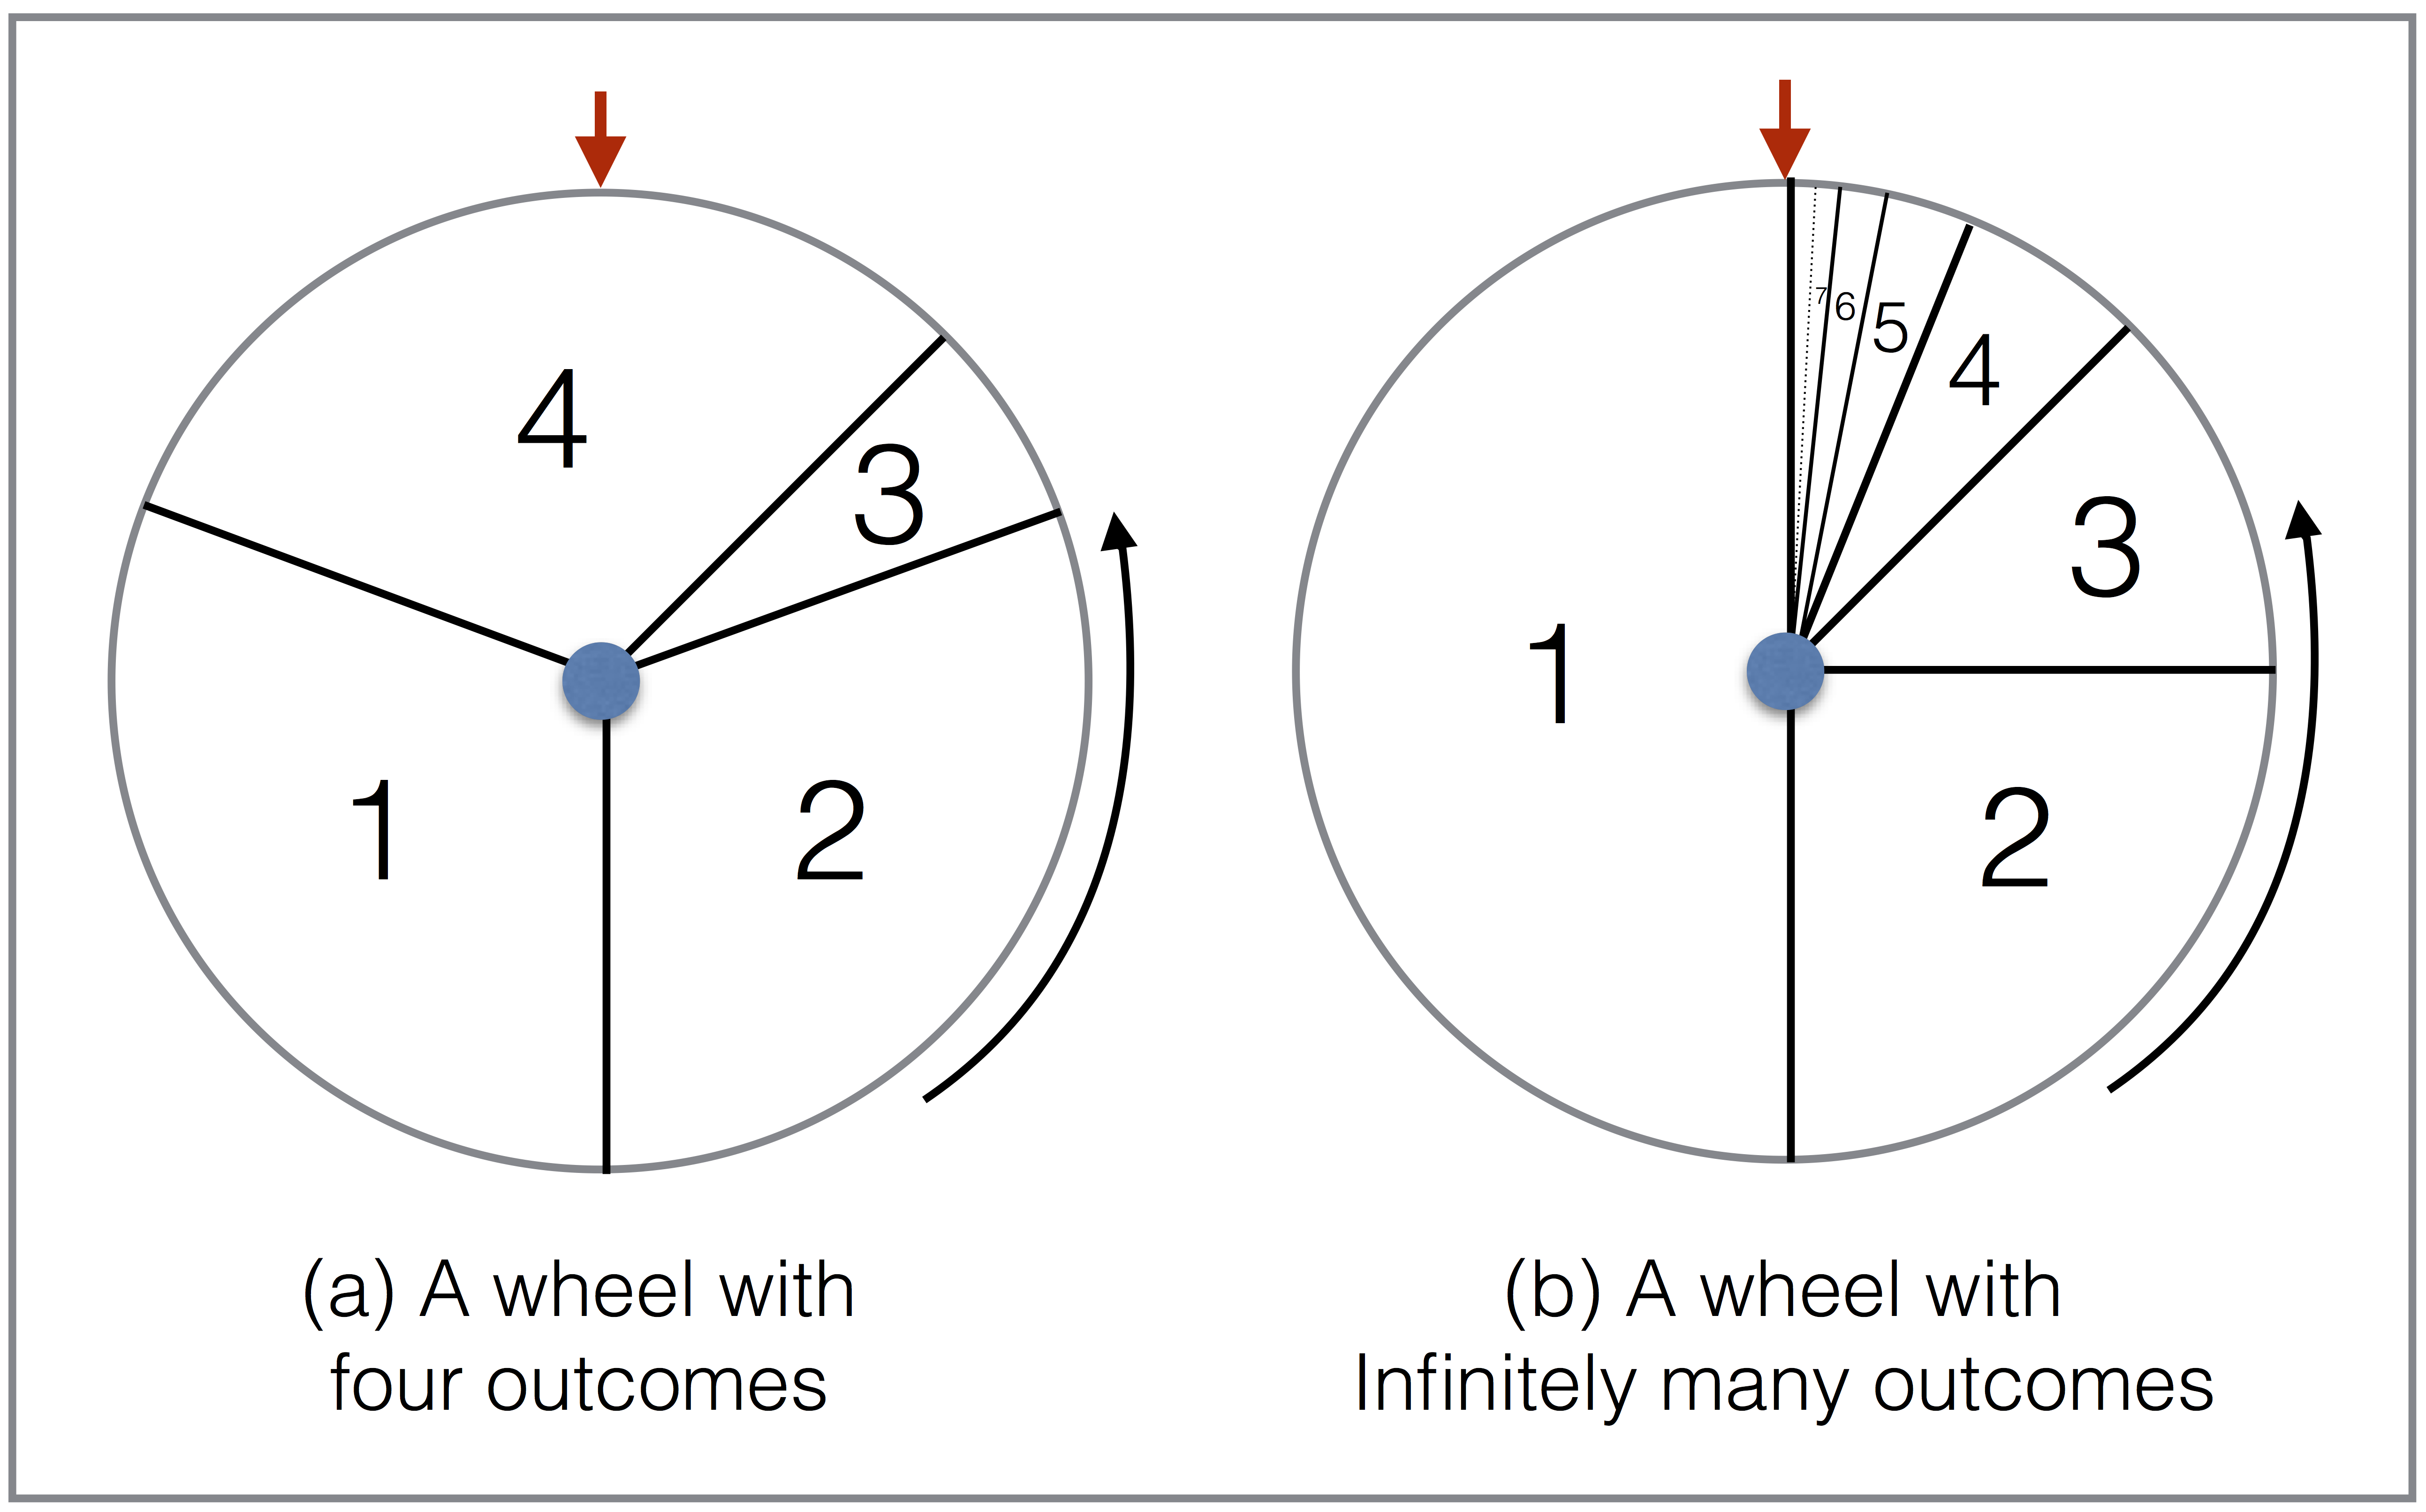
\includegraphics[width=5in]{figs/WheelsOfChanceFiniteCoutable.png}
\end{center}
\caption{Wheels of chance: the wheel is given a push and spins until
  is comes to rest. The outcome is the label of the section of the
  wheel pointed to by the red arrows. {\bf(a):} A wheel with four
  sections of different sizes. {\bf(b):} A wheel with an infinite
  number of sections, labeled with the natural numbers $1,2,3,ldots$.
\label{fig:Wheel-of-chance}}
\end{figure}

%Akshay: I'm not sure what it means to work in the rotating wheel here, since random variables and their expectations (i.e. bets) haven't yet been considered, I believe.

% Yoav: at this point the spinning wheel is just a mechanism for
% generating outcomes (elements of \Omega). The power of this
% mechanism is that it can be used to explain non-uniform discrete 
% distributions, density distributions, and even mixtures of the two.

We showed how the distribution over a finite sample space can be
specified by specifying the probability of each outcome.

What about infinite sets? Well, that depends on how ``infinite'' the set is.

As this is not a course on set theory, we will restrict our attention
to the two most useful ones, which we will describe on an intuitive
level, rather than formally. The two types of infinity that we will
consider are:
\begin{enumerate}
\item {\bf The natural numbers} The set of all natural numbers:
  $1,2,3,\ldots$ is obviously infinite. However, it is a ``small''
  type of infinite because it is {\em countable}. This means that you
  can put all of the numbers in a list.
\item{\bf The real numbers} Consider the set of points on a line, or
  even just the points on a short line segment. For example, suppose 
\[ \Omega = \left\{x | 0 \leq x \leq 1 \right\} \].
  As it turns out, the elements of this set {\em cannot} be put
  on a list, in other words, this set is not countable. As we will
  see, this means that tools from calculus are needed to define
  probability distributions on this set.
\end{enumerate}

We start with the smaller infinity, the countable infinity of the natural numbers.

\section{Distributions over the natural numbers}
Following the example of Figure~\ref{fig:Wheel-of-chance}(a) we
construct a distribution over the natural numbers using the following
iteration (depicted in part (b) of Figure~\ref{fig:Wheel-of-chance}).
\begin{enumerate}
\item The outcome 1 is given the probability $p_1=1/2$ by assigning it a
  slice that occupies $360/2 = 180$ degrees.
\item The outcome 2 is given the probability $p_2=(1/2)^2=1/4$ by
  assigning it a slice that occupies $360/4=90$ degrees. 
\item The outcome 3 is given the probability $p_3=(1/2)^3=1/8$ by
  assigning it a slice that occupies $360/8=45$ degrees.
\item ...
\item The outcome $i$ is given probability $p_i=(1/2)^i$ by assigning to
  it a slice that occupies $360/2^i$ degrees. 
\end{enumerate}

How do we know that this scheme works? In other words, how do we know
that the sum of the probabilities of all of the outcomes sums to 1?

Consider the fraction of the probability that remains after the first
$n$ outcomes have been assigned. It is not hard to convince yourself
that this remaining probability is exactly twice $p_{n+1}$ (if you
want a formal proof, try induction!):
\[
1-\sum_{i=1}^n p_i = 1-\sum_{i=1}^n (1/2)^i = (1/2)^n= 2p_{n+1}
\]
Thus each additional element halves the remaining probability. If we
repeat this for all $i$ in the natural numbers we converge, in the
limit to $1$. This is written in the following way
\[
\sum_{i=1}^{\infty} p_i = \sum_{i=1}^{\infty} (1/2)^i = 1
\]

This is our first example of a {\em convergent series} - an infinite
sequence of non-zero numbers whose sum is finite. We will use
convergent sequences later in the book, when we discuss the expected
value of a random variables. For now, we give a brief overview of
convergent and divergent sequences.

To start, the example given above is an example of a {\em geometric
  series}. The formula for the geometric series is 
\[
\sum_{i=1}^{\infty} r^i = \frac{r}{1-r}
\]
where $r$ is a real number between $0$ and $1$. 
The scheme described in the figure corresponds to $r=1/2$.

Notice that the series is infinite, but it evaluates to a finite value. 
This can happen if the sum is a geometric series. 

However, other series have this property as well. 
One that will be useful to us is the series
$$ \sum_{i=1}^\infty \frac{1}{i^2} = \frac{\pi^2}{6} $$
%(Determining the value of this series was a famous mathematical problem for decades, called the Basel problem.)
Therefore, the distribution $p_i = \frac{6}{\pi^2 i^2}$ is valid, because $ \frac{6}{\pi^2} \sum_{i=1}^\infty \frac{1}{i^2} = 1 $.

Of course, infinite series can evaluate to infinity as well. 
A well-known example we will use is the \emph{harmonic series}
$$ \sum_{i=1}^\infty \frac{1}{i} $$

\section{Tossing a biased coin}
\label{sec:BaisedCoin}

Suppose that instead of a fair coin, you have a coin whose probability of coming up heads is $p \in [0,1]$. The sample space for a single coin toss is $\Omega_o = \{H,T\}$ and the probabilities of the possible outcomes are
$$ \pr(H) = p, \ \ \pr(T) = 1-p.$$

If you toss this coin $n$ times (sample space $\Omega = \{H,T\}^n$), what is the chance of getting exactly $k$ heads? Well, pick any sequence $\omega \in \Omega$ with $k$ heads. The probability of getting precisely the outcome $\omega$ is
$$ \pr(\omega) = p^k (1-p)^{n-k} .$$
Thus the probability of $k$ heads is
$$ \mbox{(number of sequences with $k$ heads)} \cdot p^k (1-p)^{n-k} 
\ \ = \ \ 
{n \choose k} p^k (1-p)^{n-k} .$$

Sometimes we encode heads and tails numerically:
$$ \mbox{heads} \rightarrow 1, \ \ \ \mbox{tails} \rightarrow 0 .$$

In this case, a single coin flip with bias $p$ has sample space $\{0,1\}$ and is called a Bernoulli($p$) distribution. Suppose $n$ such coins are flipped, and $X_i \in \{0,1\}$ is the outcome for the $i$th coin. Then the number of heads is simply 
$$ X = X_1 + X_2 + \cdots + X_n. $$
$X$ has sample space $\{0,1,\ldots,n\}$ and is said to have a Binomial($n,p$) distribution.


\section{Density distributions}

\begin{figure}[th]
\begin{center}
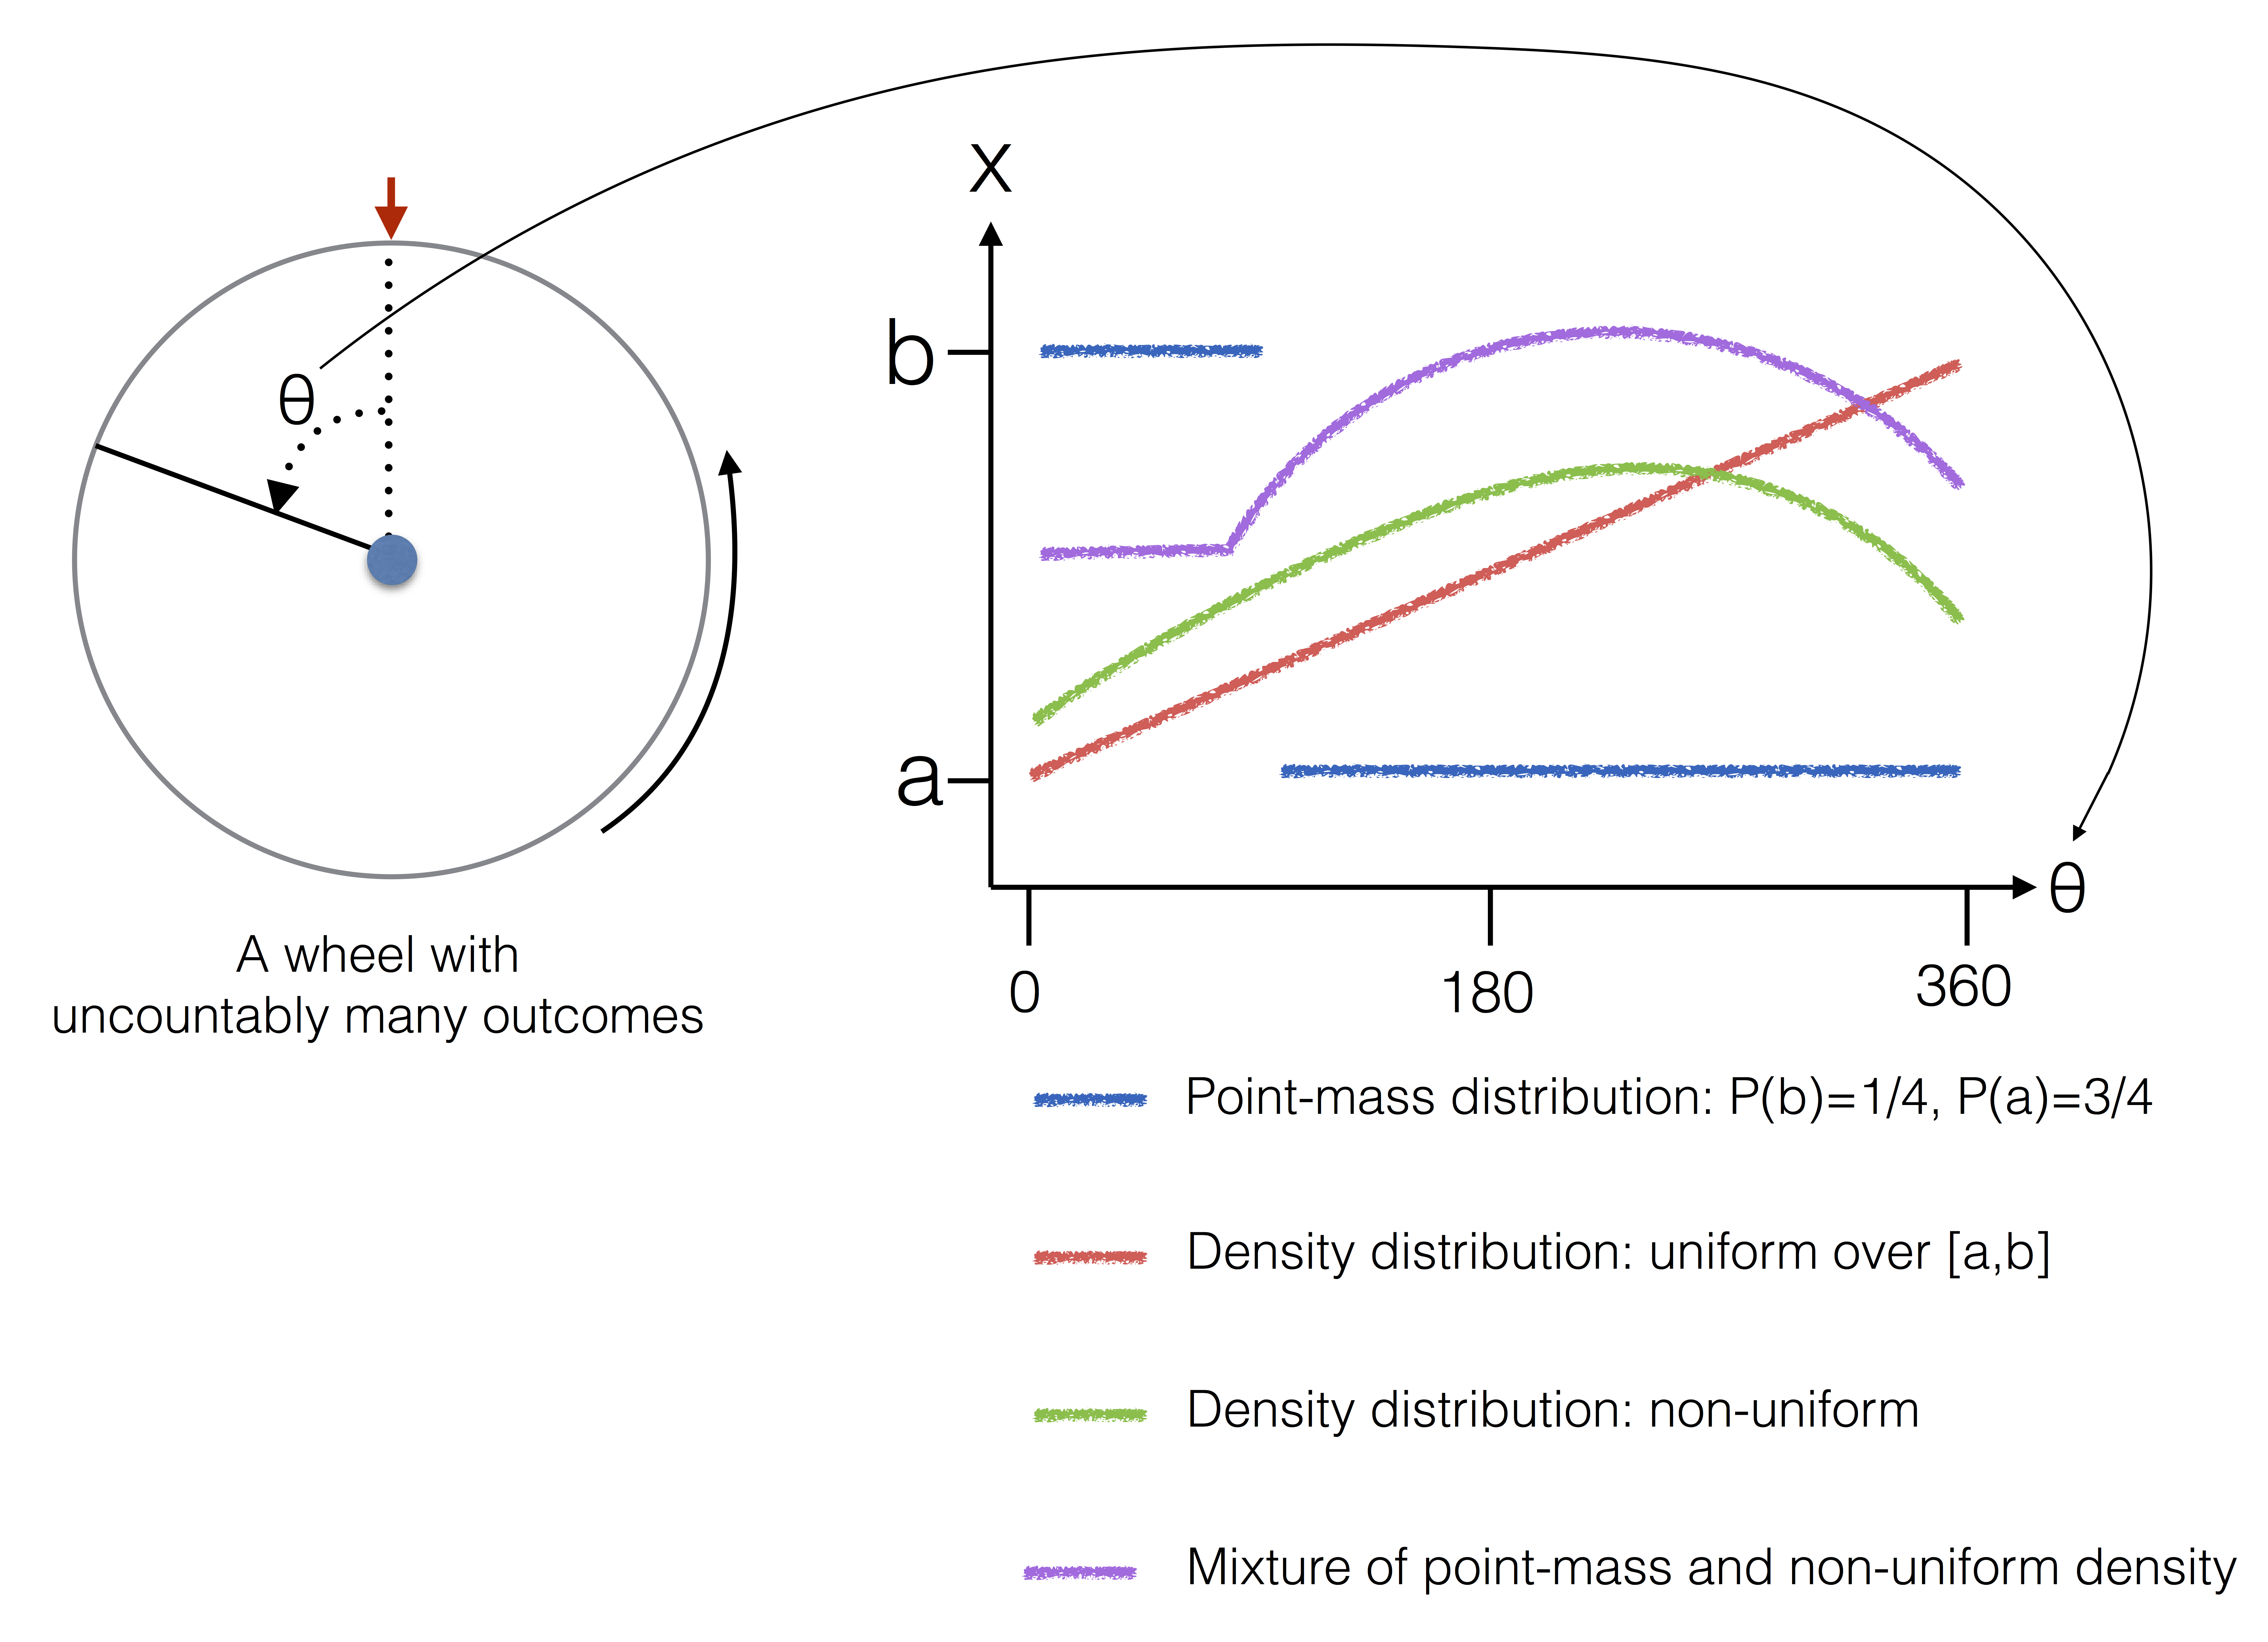
\includegraphics[width=5in]{figs/WheelsOfChanceUncountable.png}
\end{center}
\caption{{\bf Todo:} write a caption for the figure.
\label{fig:Wheel-of-chance-uncountable}}
\end{figure}

{\bf Todo: } 
\begin{itemize}
\item Kolmogorov's axioms of probability
\item Why a uniform distribution over the integers is impossible.
\item Why a uniform distribution over $[0,1]$ is possible: because
  Kolmogorov considers only countable unions.
\end{itemize}


\section{Mixture distributions}

{\bf Todo:} Describe.
\section{The limitations of histograms}

\begin{figure}[th]
\begin{center}
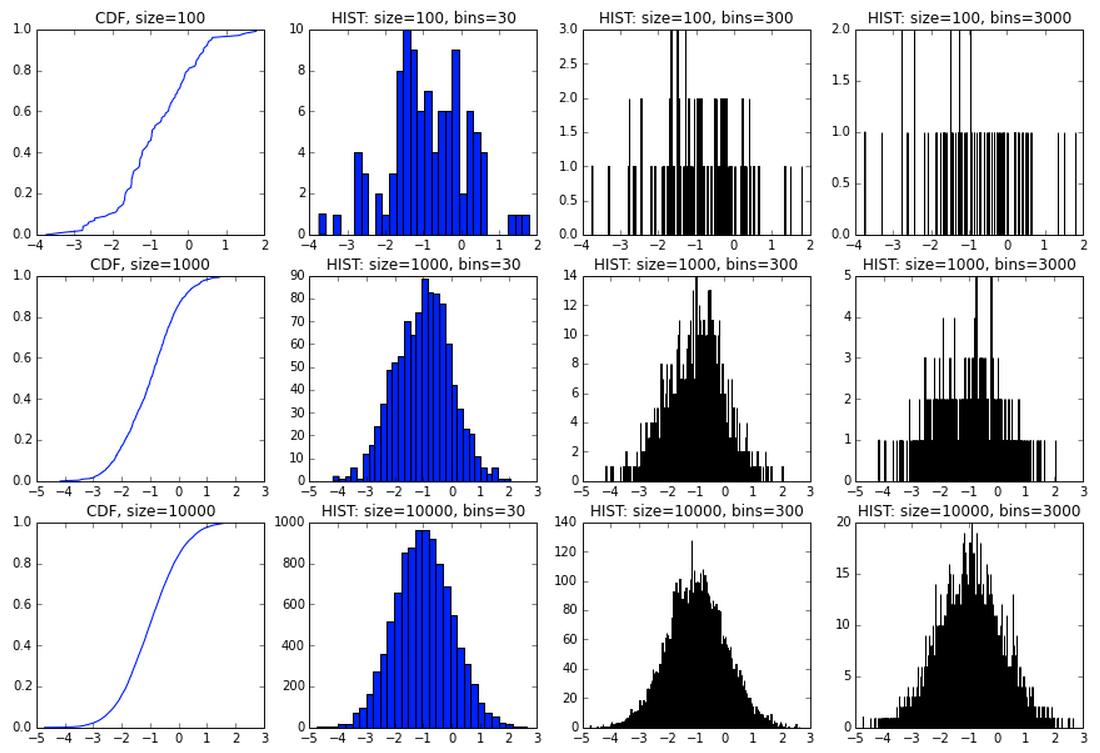
\includegraphics[width=5in]{figs/HistogramsVsCDF_D.jpg}
\end{center}
\caption{{\bf Comparison of histograms with CDF for continuous distributions:} Figure shows the effect of varying the bin width of a histogram and compares it to a CDF on the same data.\label{fig:HistogramsVsCDF_D}}
\end{figure}

\begin{figure}[th]
\begin{center}
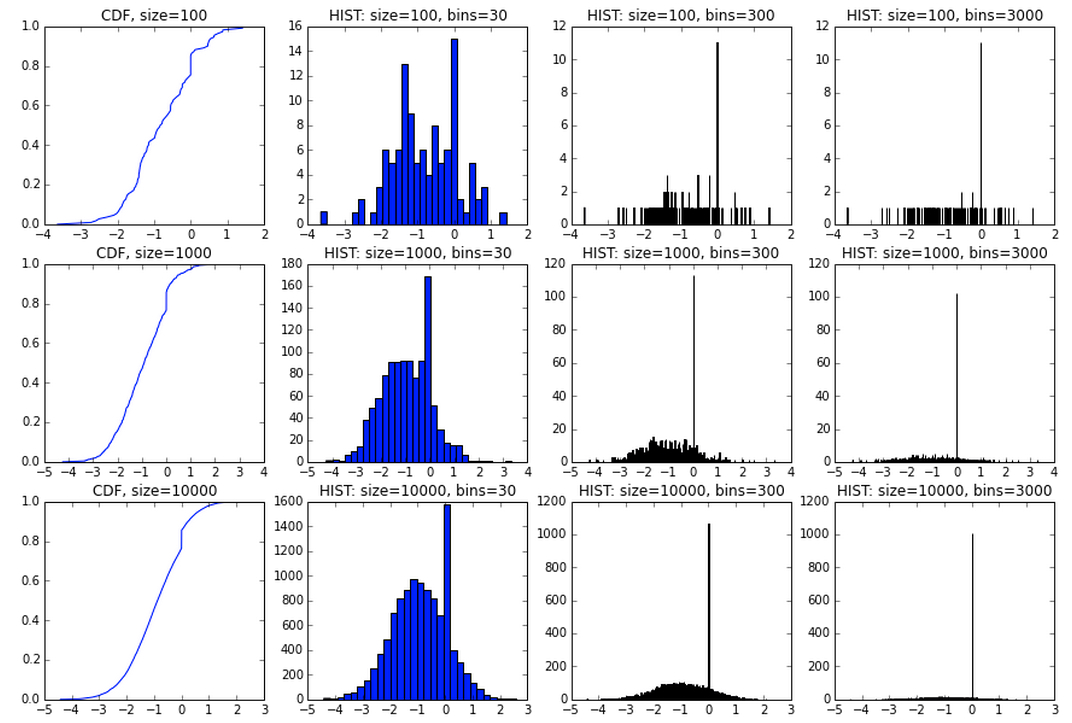
\includegraphics[width=5in]{figs/HistogramsVsCDF_PM+D.jpg}
\end{center}
\caption{{\bf Comparison of histograms with CDF for continuous distributions with a point mass:} Figure shows the effect of varying the bin width of a histogram and compares it to a CDF on the same data. \label{fig:HistogramsVsCDF_PM+D}}
\end{figure}

Figure~\ref{fig:HistogramsVsCDF_D}  and Figure~\ref{fig:HistogramsVsCDF_PM+D} show some of the limitations of using histograms.
Histograms are generated by forcing continuous data into discrete bins. While this provides an easy method to visualize the data, an incorrect choice of bin width provides little useful information.
%{\bf Todo:}Use figures to demonstrate the problems:
\begin{itemize}
\item Choosing the right width for the bins - Figure~\ref{fig:HistogramsVsCDF_D} shows the comparison between histogram and CDF for a continuous density. When there are too few bins, we lose granularity on the variation within the bin. When there are too many bins, we do not have enough data samples in each bin to accurately mirror the density. This problem is particularly accentuated when we have few samples of data. In Figure~\ref{fig:HistogramsVsCDF_D}, this scenario is shown by the histogram in the top right corner. As we move down, the number of samples increases and the histogram does a better job of representing the density. 
\item Visualizing a distribution that is a mixture of a density and a point-mass - Figure~\ref{fig:HistogramsVsCDF_PM+D} shows the challenges in the choosing the bin width when we have a distribution that is a mixture of a continuous density and a point mass. Having too many bins completely suppresses the representation of the continuous density in the histogram and accentuates the point mass. This problem is accentuated with increasing data. This scenario is represented by the histogram in the bottom right corner of Figure~\ref{fig:HistogramsVsCDF_PM+D}.
\end{itemize}
The CDF on the other hand does a better job of describing the nature of the distribution.\section{Cumulative Distribution Functions}

Our discussion so far focused on finite event spaces or event spaces
that correspond to the integers $0,1,2,\ldots$ (so-called countable
infinite sets). How do we define distributions over the real numbers?
That is an {\em uncountably} infinite set.\footnote{A set $A$ is
  uncountable if there is no one-to-one mapping from $A$ to the
  positive integers $1,2,3,4,...$. In other words, a set is
  uncountable if you cannot create a list which includes all of the
  elements in the set.}

When defining a distribution over the real it is not enough to assign
probabilities to individual points on the real line. Consider the {\em
  uniform distribution on the line segment $[0,1]$}, by which
we mean the set $\{x | 0 \leq x \leq 1\}$. We cannot assign each
point a probability larger than zero. because that would result in
$[0,1]$ an infinite probability. What we do instead is assign
probability to the line segment $0 \leq a < b \leq 1$ the probability
$b-a$. Thus for example $P([1/4,1/3])=1/3-1/4 = 1/12$.

More generally, we can define any distribution over the real line
using the {\em Cumulative Distribution Function}:
\[
\CDF(a) \doteq P(x \leq a)
\]

\begin{figure}[th]
\begin{center}
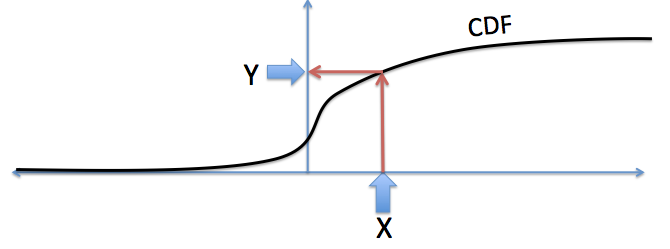
\includegraphics[width=5in]{figs/CDFmapping.png}
\end{center}
\caption{This figure depicts an example of mapping a random variable
  $X$ whose distribution is defined by a CDF (thick black curve) to
  another random variable $Y$, whose distribution is uniform in the
  interval $[0,1]$. The mapping uses the CDF as a function so that
  $Y=\CDF(X)$. \label{fig:CDFmap}}
\end{figure}

\begin{figure}[h]
\begin{center}
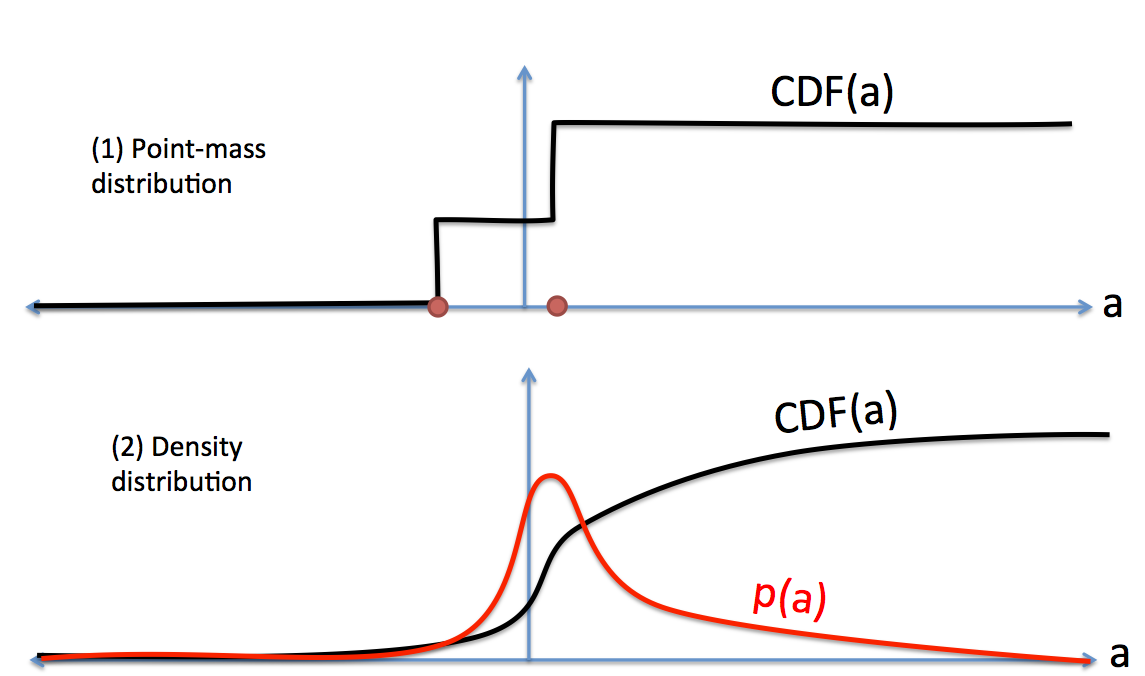
\includegraphics[width=5in]{figs/CDFs.png}
\end{center}
\caption{The CDFs for two distributions: (1) A point-mass distribution
  is a distribution that assignes non zero probabilities to two real
  values (marked by red circles) all sets that do not include at least
  one of these points have probability zero. The CDF of a point mass
  distribution is constant every where but at the point masses where
  it is discontinuous, the size of the discontinuity is the
  probability of the corresponding point. (2) A density distribution
  assigns probability zero to any single point. The CDF for such a
  distribution is a continuous increasing function that has a
  derivative. This derivative, $p(a)$ is called the {\em density function} of
  the distribution. For density distributions the CDF and the density
  function contain the same information.\label{fig:CDF}}
\end{figure}

As we see in Figure~\ref{fig:CDF} the CDF is an increasing function that
increases from zero at $-\infty$ to one at $+\infty$.

It is easy to see that $P(a<x\leq b)=\CDF(b)-\CDF(a)$.


\section{Examples of distributions on the real line}
If the distribution assigns a non-zero probability to some $x=a$ we
say that the distribution has a {\em point mass} at $a$. In that case
the $\CDF$ has a jump at $a$. We denote a point mass distribution
concentrated at the point $a$ by $PM(a)$. The distribution $PM(a)$
corresponds to a random variable such that $P(X=a)=1$.

\begin{figure}[t]
\begin{center}
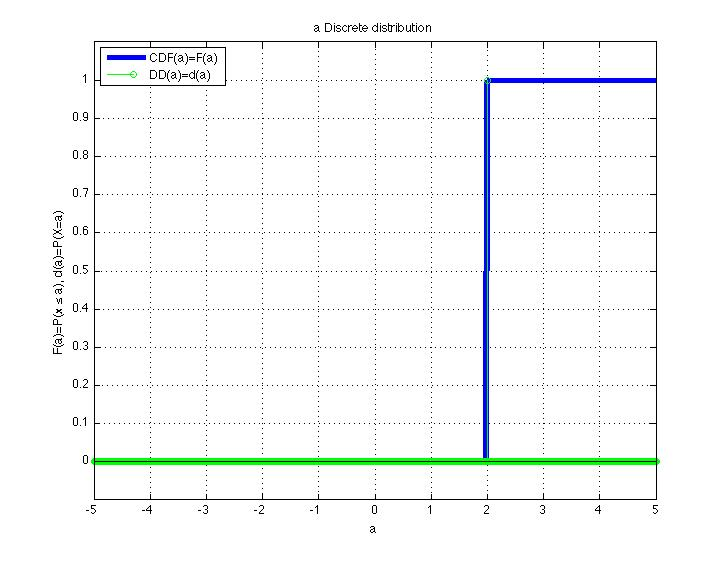
\includegraphics[width=3in]{figs/Discrete1.jpg}
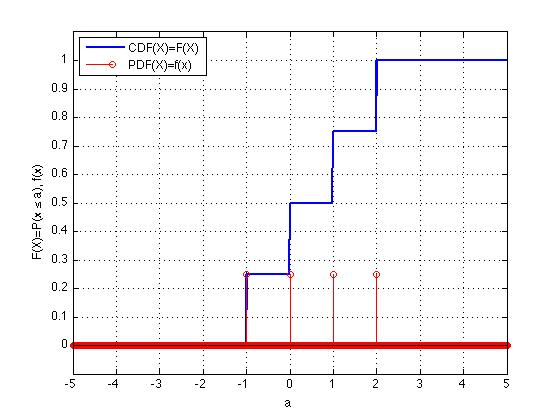
\includegraphics[width=3in]{figs/4PointMass.jpg}
\end{center}
\caption{{\bf Left:} A discrete distribution concentrated on a single
  point $P(X=2)=1$. We denote this distribution by $PM(2)$.  {\bf
    Right:} A discrete distribution distributed evenly over the four
  points $-1,0,1,2$. This distribution can be expressed as $(PM(-1)+PM(0)+PM(1)+PM(2))/4$.}
\end{figure}

\begin{figure}[b]
\begin{center}
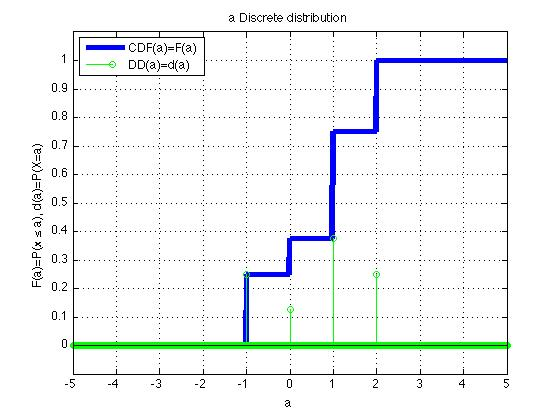
\includegraphics[width=3in]{figs/Discrete2.jpg}
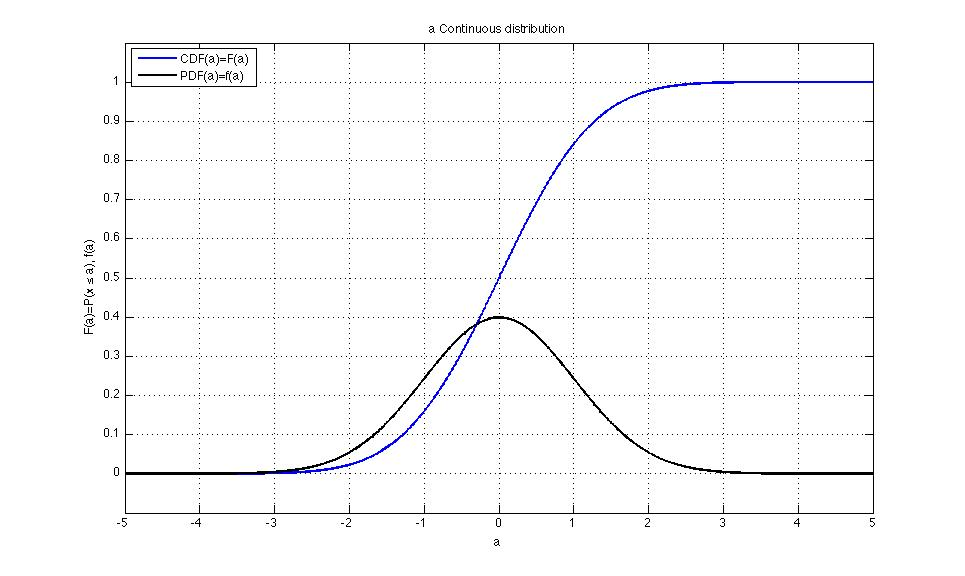
\includegraphics[width=3in]{figs/Normal.jpg}
\end{center}
\caption{{\bf Left:} A non-uniform discrete distribution. This
  distribution can be expressed as
  $(1/4)PM(-1)+(1/8)PM(0)+(5/8)PM(1)+(1/4)PM(2)$. {\bf Right:} The
  normal distribution with mean $0$ and varriance 1, denoted ${\cal
  N}(0,1)$. This is a density distribution and it's density function
is $f(x) = \frac{1}{\sqrt{2\pi}} \exp(-x^2/2)$.}
\end{figure}

\begin{figure}[t]
\begin{center}
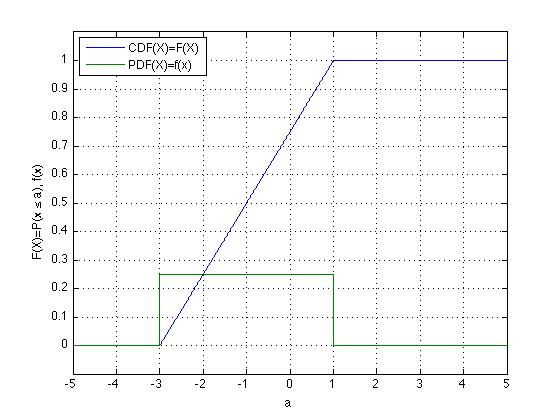
\includegraphics[width=3in]{figs/Uniform.jpg}
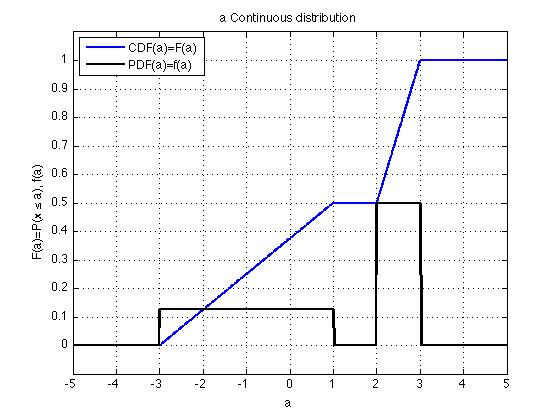
\includegraphics[width=3in]{figs/unifMixture2CDF.jpg}
\end{center}
\caption{{\bf Left:} A uniform distribution between $-3$ and $1$. We
  denote this distribution by $U(-3,1)$. {\bf Right:} A mixture of two
  uniform distributions: $(U(-3,1)+U(2,3))/2$.}
\end{figure}

\[
f(x) = \begin{cases}
0.25 & \mbox{if $ -3 \leq x \leq 1$} \\
0 & \mbox{otherwise}
\end{cases}
\]

Another important case is when the deriveative of the CDF is deifined
$p(a) = \frac{d}{dx}\left|_{x=a} \CDF(x)\right.$. The function $p(a)$
is called the {\em probability density}. Note that if $p(a)$ is
defined then, regarless of how large $p(a)$ is, $P(x=a)=0$.

When a distribution over the reals is a density distribution we can
calculate the probability of the segment $[a,b]$ using the integral:
\[
P(a < x \leq b)=\CDF(b)-\CDF(a)=\int_a^b p(x) dx
\]

\section{Throwing a dart at a dartboard} 
%{\bf todo:} Add an image of a dartboard.
\begin{figure}[H]
\begin{center}
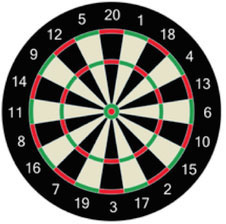
\includegraphics[width=1in]{figs/dartboard.jpg}
\end{center}
\caption{{\bf Dartboard}
 \label{fig:Dartboard}}
\end{figure}


Suppose for convenience that your dartboard has radius 1, and is
centered at the origin. Its bullseye has radius 0.1. You throw a dart
at it, which lands at a random location (all positions on the board
are equally likely). What is the chance that it lands exactly at the
origin? What is the chance that it lands in the bullseye?

This differs from earlier examples in that the sample space is infinite and continuous. It is the set of all possible locations of the dart: any point in the circle. We can represent any such point by its $(x,y)$ coordinates: $\Omega = \{(x,y): x^2 + y^2 \leq 1\}$.

The chance of landing exactly at the origin is 0, since there are infinitely many places the dart could land. It makes more sense to talk about landing in {\it regions} $A \subset \Omega$ rather than specific points $\omega \in \Omega$. In general
$$ \pr(A) = \frac{\mbox{area of $A$}}{\mbox{area of $\Omega$}} $$
and therefore $\pr(\mbox{bullseye}) = (0.1)^2 = 0.01$.

{\bf Todo:} Use $x,y$ and $r$-the distance from the bullseye, 
as examples of random variables.



